\section{Final remarks}

\begin{frame}
  Final remarks.
\end{frame}

\begin{frame}
  \frametitle{Final remarks}
  \begin{itemize}
    \item Please wonder if it is worth it to learn these tools, especially if
      you are going to be doing science \textbf{for the rest of your life}.
    \item Check
      \href{https://sites.unipampa.edu.br/sisbi/files/2023/08/manualzotero_versoafinal.pdf}
      {here} the \textit{Tutorial para gerenciamento de referências
      bibliográficas utilizando o software Zotero} by the Ibict.
    \item There is a check list for submissions to TREESLab's Zenodo community
      (check it \href{https://docs.google.com/document/d/18ZKzcsP6GazzO0X5FDE8FUfkehaD3X3hoxrnWLSxI8o/edit?usp=sharing}
          {here}).
    \item Also, check TREESLab' Discord chanels:
    \begin{itemize}
      \item \href{https://discord.com/channels/1207666629454856192/1215297398343999619}
      {ajuda-zotero}.
      \item \href{https://discord.com/channels/1207666629454856192/1215297581437947984}
        {ajuda-zenodo}.
    \end{itemize}
  \end{itemize}
\end{frame}

\begin{frame}
  \frametitle{RTFM}
  \begin{columns}
    \begin{column}{0.5\textwidth}
      \begin{itemize}
        \item Users don't acknowledge RTFM as their first option to solve
        software problems.
        \item This is so common, that software developers created RTFM as a
        gentle reminder to users of their options when dealing with software
        they don't know (check Wikipedia's article
        \href{https://en.wikipedia.org/wiki/RTFM}{about it}).
      \end{itemize}
    \end{column}
    \begin{column}{0.5\textwidth}
      \begin{figure}
        \centering
        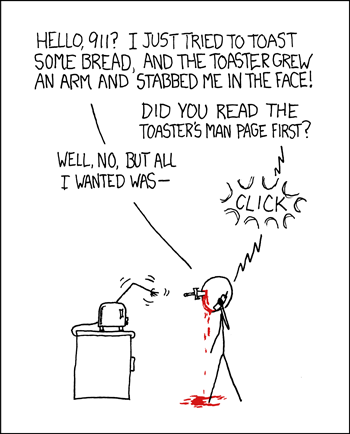
\includegraphics[scale=0.4]{images/rtfm.png}
        \caption{Source: RTFM by \href{https://imgs.xkcd.com/comics/rtfm.png}{xkcd}.}
      \end{figure}
    \end{column}
  \end{columns}
\end{frame}
